\section{Response to Reviewer \#2}

Dear Reviewer 2,\\

Thank you very much for your positive feedback and insightful comments on our manuscript. We appreciate the reviewer's recognition that the combination of MDS-coded diversity transforms with polar codes is a promising direction. Your constructive suggestions have helped us strengthen the technical contributions and presentation. We provide our detailed responses below.

\noindent\rule{17cm}{2.0pt}

%%%%%%%%%%%%%%%%%%%%%%%%%%%%%%%%%%%%%%%%%%%%%%%%%%%%%%%%%%%%%%%%%%%%%%
\subsection{Reviewer Comment-1}



\begin{mdframed}
\begin{quote}

The paper introduces a diversity transform framework integrated with OTFS modulation to improve link reliability in LEO NTN downlinks without relying on retransmissions. The authors derive finite-blocklength BLER expressions under Rician fading and propose an ephemeris-driven outage prediction mechanism. The combination of MDS-coded diversity transforms with polar codes is a promising direction. However, several significant issues must be addressed.
1. The paper compares against “standalone FEC” and “FEC with interleaving”. However, existing satellite diversity methods such as maximal ratio combining (MRC), selection combining (SC), and HARQ with chase combining are only briefly mentioned in the introduction. No quantitative comparison with MRC/SC-based multi-connectivity is provided in the numerical results. The authors could include a baseline that uses MRC across subchannels (without the diversity transform) and show the BLER vs. SNR or blockage probability.

\end{quote}

\end{mdframed}


\subsection{Response}

We thank the reviewer for this suggestion. In the revised manuscript, quantitative MRC and SC baselines have been added to both the latency comparison (Fig.~\ref{fig:latency_comparison}) and the throughput comparison (Fig.~\ref{fig:throughput}). MRC combines LLRs from all non-blocked subchannels while SC selects the best subchannel; both repeat the same codeword on every subchannel and therefore require $k_c = 4$ times more channel uses for the same message. The diversity transform achieves the lowest latency at every operating point, and in throughput, it surpasses rate-optimised MRC at $P_{\mathrm{total}} \approx 12$~dBW and achieves nearly twice the MRC throughput at 25~dBW. A direct BLER-versus-SNR comparison was not included because equalising both message size and total channel uses would require MRC to operate at a code rate exceeding unity, which is unrealisable; the latency and throughput comparisons normalise for this resource difference. MRC and SC baselines have been added to the latency comparison (Fig.~\ref{fig:latency_comparison}) alongside HARQ-CC:

\begin{quote}
``{\color{blue}Fig.~\ref{fig:latency_comparison} demonstrates the latency advantage of the diversity transform over MRC, SC, and the HARQ-CC baseline$\ldots$ MRC combines LLRs from all non-blocked subchannels (effective SNR $= \sum_j \bar{\gamma}_j$), and SC selects the subchannel with the highest instantaneous SNR; both repeat the same codeword on every subchannel and therefore require $k_c$ times more channel uses to deliver the same message size.}''
\end{quote}

\begin{center}
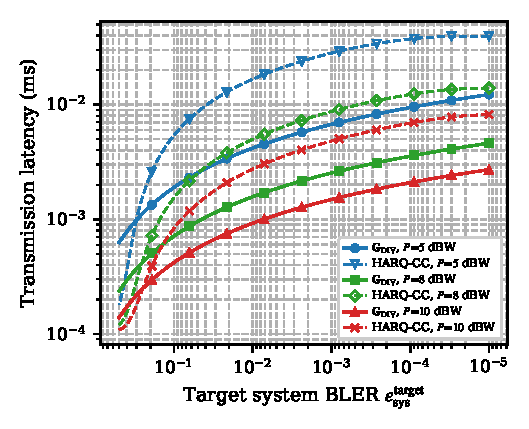
\includegraphics[width=0.7\columnwidth]{latency_comparison.eps}\\
{\small \textbf{Fig.~\ref{fig:latency_comparison}:} {\color{blue}Transmission latency versus target system BLER $\epsilon_{\mathrm{sys}}^{\mathrm{target}}$ for the diversity transform, MRC, SC, and HARQ-CC ($K_{\max} = 4$, $T_{\mathrm{RTT}} = 20$~ms) at $P_{\mathrm{total}} = 5$ and $10$~dBW. MRC and SC require $k_c = 4$ times more channel uses to deliver the same message size.}}
\end{center}

The throughput comparison in Section~V now reads:

\begin{quote}
``{\color{blue}$\ldots$ Rate-optimised MRC and SC are also included. Both schemes repeat the same codeword on all $n_{\mathrm{s}}$ subchannels, giving throughput $\eta_{\mathrm{MRC/SC}} = (R/n_{\mathrm{s}}) \cdot (1 - \epsilon)$, where $R$ is optimised at each operating point to maximise throughput given the combined SNR ($\gamma_{\mathrm{MRC}} = \sum_j \gamma_j$ for MRC, $\gamma_{\mathrm{SC}} = \max_j \gamma_j$ for SC). Despite adaptive rate optimisation, MRC and SC saturate at approximately $0.16$~bits per channel use because of the $1/n_{\mathrm{s}}$ repetition penalty. $\ldots$ The diversity transform surpasses rate-optimised MRC at $P_{\mathrm{total}} \approx 12$~dBW and achieves nearly twice the MRC throughput at $25$~dBW.}''
\end{quote}

\begin{center}
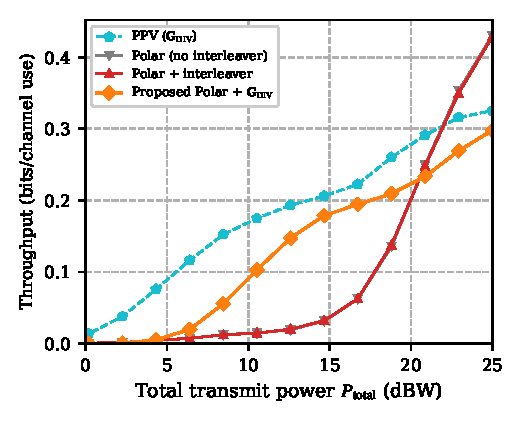
\includegraphics[width=0.7\columnwidth]{throughput_reliability.eps}\\
{\small \textbf{Fig.~\ref{fig:throughput}:} {\color{blue}Effective throughput versus total transmit power at $\epsilon = 40^{\circ}$ with $n_{\mathrm{s}} = 6$ subchannels. The diversity transform operates at effective rate $R_c \cdot \varrho/n_{\mathrm{out}} \approx 0.33$; per-subchannel baselines at $R_c = 0.5$. MRC and SC are rate-optimised at each power level.}}
\end{center}

A direct BLER-versus-SNR comparison was not included because MRC and SC repeat the same codeword on all $n_{\mathrm{s}}$ subchannels, consuming $n_{\mathrm{s}}$ times more channel uses for the same message. Equalising both message size and total channel uses would require MRC to operate at a code rate of $k_{\mathrm{c}} \cdot R_c = 2.0 > 1$, which is unrealisable. The latency and throughput comparisons normalise for this resource difference and provide the appropriate evaluation.

We trust that the new latency and throughput comparisons provide the quantitative MRC/SC evaluation requested.


\subsection{Reviewer Comment-2}



\begin{mdframed}
\begin{quote}

The proposed prediction framework in Section III-B relies on perfect ephemeris knowledge and assumes negligible UE location error. No sensitivity analysis is provided for ephemeris errors, UE positioning inaccuracies, or atmospheric model mismatches.
3. Theorem 1 and Proposition 1 assume: Perfect channel estimation at the receiver; No fractional Doppler (integer Doppler indices only); Ideal MRC combining in the DD domain. These assumptions are not fully justified for LEO NTN scenarios, where fractional Doppler is common and channel estimation errors are non-negligible.

\end{quote}

\end{mdframed}


\subsection{Response}

We thank the reviewer for raising these points. We agree that these assumptions needed to be relaxed and quantified. In the revised manuscript, two new analytical models and four new simulation results address both concerns: (i) a prediction robustness analysis in Section~IV-E models the combined error from ephemeris, UE location, and atmospheric mismatch as a log-normal perturbation $\sigma_p$, with a new Proposition providing the closed-form BLER under imperfect prediction and two new figures (Figs.~\ref{fig:bler_robustness} and~\ref{fig:latency_robustness}) confirming graceful degradation up to $\sigma_p = 4$~dB; and (ii) a SINR impairment model in Section~II-C captures fractional Doppler and imperfect channel estimation, with two new curves in Fig.~\ref{fig:otfs_vs_ofdm} showing that the OTFS advantage over OFDM is preserved under realistic impairments (BLER increase of approximately $1.5$--$2$ times). Regarding prediction sensitivity, a new subsection, Section~IV-E, ``Sensitivity to Prediction Imperfections,'' has been added:

\begin{quote}
{\color{blue}
\subsection{Sensitivity to Prediction Imperfections}

The prediction framework in Section~\ref{sec:ephemeris_prediction}
assumes perfect ephemeris knowledge and accurate UE positioning.
In practice, three sources of uncertainty introduce discrepancies
between the predicted and actual subchannel SNRs:
(i)~orbital ephemeris errors, which produce elevation-angle
offsets propagating through the slant-range
and atmospheric-loss models in~\eqref{eq:predicted_path_loss};
(ii)~UE location uncertainty, which introduces additional
elevation-angle error; and
(iii)~atmospheric model mismatch, arising from real-time
variability in tropospheric and ionospheric conditions that
deviates from the statistical models used
in~\eqref{eq:predicted_path_loss}.  The combined prediction error for subchannel~$i$ is represented as $\delta_i \sim \mathcal{N}(0, \sigma_p^2)$, where $\sigma_p$~(dB) characterises the aggregate uncertainty. Incorporating this prediction error, the predicted end-to-end SNR for subchannel~$i$ is modelled using the following log-normal multiplicative perturbation model~\cite{Papoulis2002}:
\begin{equation*}
\check{\gamma}_i^{\mathrm{E2E}} =
\gamma_i^{\mathrm{E2E}} \cdot 10^{\delta_i/10},
\end{equation*}
where $\delta_i$ are assumed mutually independent across subchannels.

Under~\eqref{eq:snr_mismatch}, the erasure declaration and
reliability scoring from Section~\ref{sec:ephemeris_prediction}
operate on the mismatched SNR $\check{\gamma}_i^{\mathrm{E2E}}$
rather than the actual $\gamma_i^{\mathrm{E2E}}$.
This introduces two types of misclassification:
a false erasure, where a reliable subchannel
($\gamma_i^{\mathrm{E2E}} \geq \psi_i$) is declared in outage
because $\check{\gamma}_i^{\mathrm{E2E}} < \psi_i$,
unnecessarily consuming MDS redundancy;
and a missed outage, where a degraded subchannel
($\gamma_i^{\mathrm{E2E}} < \psi_i$) is declared reliable
because $\check{\gamma}_i^{\mathrm{E2E}} \geq \psi_i$,
allowing corrupted soft information to enter the FEC decoder.

\noindent\textbf{Proposition~\ref{prop:bler_imperfect} (BLER Under Imperfect Prediction).}
Under the prediction error model~\eqref{eq:snr_mismatch}
and the dominant feeder-link approximation,
the prediction-error-conditioned BLER for subchannel~$i$ is
\begin{equation*}
\check{\epsilon}_i^{\mathrm{E2E}}(\sigma_p)
= \mathbb{E}_{\delta_i}\!\left[
\Upsilon\!\left(L_i - 1,\;
\frac{\left(\psi_i\cdot 10^{-\delta_i/10}
  - \gamma_{i,0}^{\mathrm{det}}\right)^{+}}
{\hat{\gamma}_{i,\mathrm{NLOS}}}\right)\right],
\end{equation*}
where $(x)^{+} \triangleq \max(x,0)$,
$\psi_i = 2^{R_c} - 1$, and the expectation is over
$\delta_i$.
Setting $\sigma_p = 0$
recovers~\eqref{eq:bler_cdf_combined}.
The system BLER under imperfect prediction follows from
Corollary~\ref{cor:sys_bler_poisson} with
$\epsilon_i^{\mathrm{E2E}}$ replaced by
$\check{\epsilon}_i^{\mathrm{E2E}}(\sigma_p)$:
\begin{equation*}
\check{\epsilon}_{\mathrm{sys}}(\sigma_p)
\approx \sum_{j=f_{\max}+1}^{n}
\tilde{P}(F = j;\,\sigma_p),
\end{equation*}
where $\tilde{P}(F = j;\,\sigma_p)$ is evaluated via the
Poisson binomial recursion~\eqref{eq:poisson_binom_recursive}
with parameters
$\{\check{\epsilon}_i^{\mathrm{E2E}}(\sigma_p)\}_{i=1}^{n}$.

\begin{IEEEproof}
{\color{blue}See Appendix~\ref{app:proof_bler_imperfect}.}
\end{IEEEproof}

The resulting impact of prediction imperfections on transmission latency
follows directly from
Corollary~\ref{cor:latency_reduction}.
Under imperfect prediction, the relaxed per-subchannel
target $\check{\epsilon}^{*}(\sigma_p)$ is obtained by
inverting~\eqref{eq:sys_bler_imperfect}:
\begin{equation*}
\sum_{j=f_{\max}+1}^{n}
\tilde{P}(F=j;\,\sigma_p)\big|_{\check{\epsilon}_i^{\mathrm{E2E}}
= \tilde{\epsilon}^{*}\;,\forall\, i}
= \epsilon_{\mathrm{sys}}^{\mathrm{target}}.
\end{equation*}
Since prediction uncertainty generally increases the effective per-subchannel failure probability, i.e.,
$\check{\epsilon}_i^{\mathrm{E2E}}(\sigma_p) \geq
\epsilon_i^{\mathrm{E2E}}$, the relaxed target satisfies
$\check{\epsilon}^{*}(\sigma_p) \leq \epsilon^{*}$,
and the minimum blocklength
from~\eqref{eq:min_blocklength_div} increases to
\begin{equation*}
\check{n}_c^{*}(\sigma_p)
= \frac{V(\gamma)\bigl[Q^{-1}
(\check{\epsilon}^{*}(\sigma_p))\bigr]^2}
{(C(\gamma) - R_c)^2}
\geq n_c^{*}(\epsilon^{*}, \gamma),
\end{equation*}
yielding a corresponding increase in the frame duration
$\check{T}_{\mathrm{frame}}(\sigma_p) =
\check{n}_c^{*}(\sigma_p)/(M_{\mathrm{D}}\Delta f)$.
}% end blue
\end{quote}

Fig.~\ref{fig:bler_robustness} shows that the system BLER degrades gracefully with increasing $\sigma_p$, with all diversity transform curves remaining well below the no-diversity baseline. Fig.~\ref{fig:latency_robustness} confirms that the latency advantage over HARQ-CC is preserved even at $\sigma_p = 4$~dB.

\begin{center}
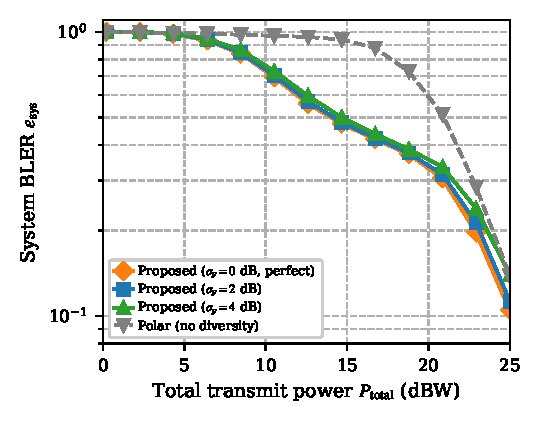
\includegraphics[width=0.7\columnwidth]{bler_robustness_prediction.eps}\\
{\small \textbf{Fig.~\ref{fig:bler_robustness}:} {\color{blue}System BLER versus total transmit power under imperfect prediction with combined prediction error $\sigma_p$.}}
\end{center}

\begin{center}
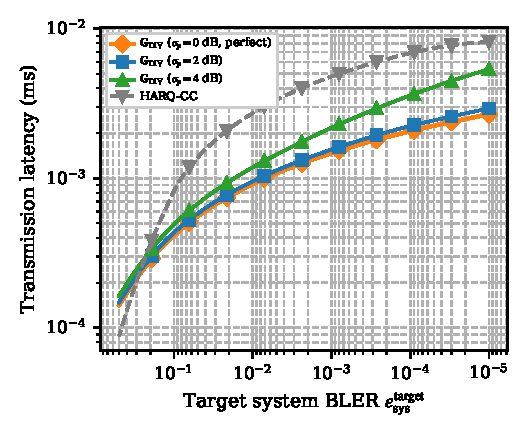
\includegraphics[width=0.7\columnwidth]{latency_robustness_prediction.eps}\\
{\small \textbf{Fig.~\ref{fig:latency_robustness}:} {\color{blue}Transmission latency versus target system BLER under imperfect prediction at $P_{\mathrm{total}} = 10$~dBW.}}
\end{center}

Regarding fractional Doppler and imperfect channel estimation, a new SINR impairment model has been added at the end of the OTFS Modulation subsection, Section~II-C:

\begin{quote}
``{\color{blue}The DD input--output relation in~\eqref{eq:dd_io} assumes
that each tap's Doppler shift aligns exactly with an integer DD bin.
When the physical Doppler $\nu_p$ of the $p$th tap does not coincide
with a grid point, a fractional offset
$\alpha_p = \nu_p - \lfloor\nu_p\rceil$ introduces inter-Doppler
interference with variance
$\sigma_{\mathrm{frac}}^2 = (\pi\,\alpha_p)^2/(3\,N_{\mathrm{D}})$~\cite{Raviteja2018,Moose1994}.
Under imperfect channel estimation with per-element MSE
$\sigma_{\mathrm{CSI}}^2$, the effective post-equalisation SINR is}
\begin{equation*}
\color{blue}
\gamma_i^{\mathrm{eff}} =
\frac{\gamma_i^{\mathrm{c}}}
{1 + \gamma_i^{\mathrm{c}}
\left(\sigma_{\mathrm{frac}}^2
+ \sigma_{\mathrm{CSI}}^2\right)}.
\end{equation*}
{\color{blue}Setting $\alpha_p = 0$ and $\sigma_{\mathrm{CSI}}^2 = 0$
recovers the ideal integer-Doppler, perfect-CSI case.}''
\end{quote}

The following discussion has been added to Section~V:

\begin{quote}
``$\ldots$ These results confirm that DD domain processing with OTFS, combined with the proposed diversity transform, is well suited to the high Doppler shifts characteristic of LEO satellite links.
{\color{blue}To quantify the impact of fractional Doppler and imperfect
channel estimation, Fig.~\ref{fig:otfs_vs_ofdm} also includes the
proposed OTFS scheme under two additional impairment conditions:
(i)~fractional Doppler with worst-case offset $\alpha_p = 0.5$ and perfect channel estimation; and
(ii)~fractional Doppler combined with imperfect channel estimation
($\sigma_{\mathrm{CSI}}^2 = 0.01$, corresponding to a channel estimation MSE of $-20$~dB, which is representative of embedded pilot-aided OTFS estimation at moderate SNR~\cite{Raviteja2018}).
Both impaired OTFS curves exhibit a moderate BLER increase (approximately
$1.5$--$2$ times) relative to the ideal integer-Doppler case, yet
remain significantly below the OFDM curves at high normalised Doppler.
This confirms that the OTFS advantage over OFDM is preserved under
realistic impairments, and that the diversity transform's
subchannel-level recovery guarantee of Theorem~\ref{thm:block_mds}
remains effective.}

\begin{center}
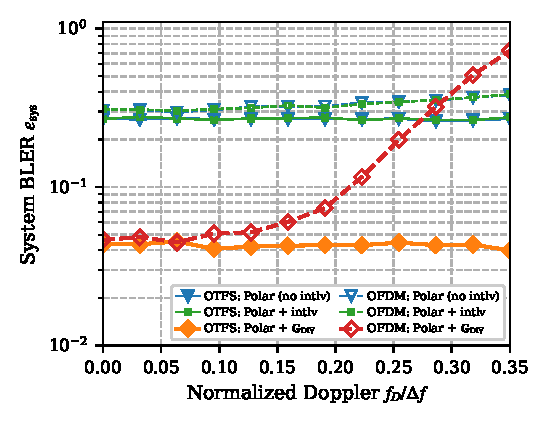
\includegraphics[width=0.7\columnwidth]{otfs_vs_ofdm.eps}\\
{\small \textbf{Fig.~\ref{fig:otfs_vs_ofdm}:} {\color{blue}BLER versus normalised Doppler $f_{D}/\Delta f$ for OTFS
and OFDM at $P_{\mathrm{total}} = 20$~dBW, including fractional
Doppler and imperfect channel estimation impairments.}}
\end{center}

In summary, the simulation results show that $\ldots$''
\end{quote}

These results directly quantify the performance gap: fractional Doppler and imperfect CSI increase the proposed scheme's BLER by approximately $1.5$ to $2$ times, while the OTFS advantage over OFDM and the diversity transform's recovery guarantee are both preserved.

We hope that the new prediction error model, SINR impairment model, simulation curves, and supporting figures address these concerns.


\subsection{Reviewer Comment-3}



\begin{mdframed}
\begin{quote}

It is not explained how the SCL decoder operates on the soft outputs of the diversity demapper, does it treat the combined code as a single polar code with a larger length? Or does it decode each subword independently?
\end{quote}

\end{mdframed}


\subsection{Response}

We appreciate this question. The SCL decoder decodes the original $(N,K)$ polar code in a single forward pass without any modification. The diversity demapper handles all inter-subchannel mixing beforehand and produces a standard vector of $N$ LLRs, one per coded bit, which the SCL decoder processes exactly as in a conventional polar code.

The processing chain works as follows. At the transmitter, the $K$ information bits are polar-encoded and then spread across $n_{\mathrm{out}}$ subchannels by the diversity transform $Z = G_{\mathrm{DIV}}^{\mathsf{T}} U G_{\mathrm{POL}}$. At the receiver, the diversity demapper computes max-log MAP LLRs from the channel outputs, jointly marginalising over all $2^{\varrho}$ input hypotheses in a single pass. The resulting $N$ soft LLRs are fed directly to the standard SCL decoder. In Section~\ref{subsec:receiver_demapping}:

\begin{quote}
``{\color{blue}The demapper output is a vector of $N$ soft LLRs corresponding to the polar-coded bits. These LLRs are passed to a single successive cancellation list (SCL) polar decoder that recovers all $K$ information bits from the original $(N,K)$ polar code in one forward pass. No modification to the standard SCL algorithm is required.} The combined polar--diversity generator $G_{\mathrm{PD}} = G_{\mathrm{POL}} \otimes G_{\mathrm{DIV}}$ preserves the algebraic rank guarantees throughout the decoding process without requiring bit-level interleaving.''
\end{quote}

In summary, the diversity demapper handles the inter-subchannel mixing and produces standard per-bit LLRs; the SCL decoder then operates exactly as it would for a conventional polar code, with no modification to the decoding algorithm or code length.

We trust that this clarification resolves the question about the decoder architecture.


\subsection{Reviewer Comment-4}



\begin{mdframed}
\begin{quote}

The sensitivity of the overall system BLER to this threshold should be explored. Does the MDS recovery guarantee still hold if the threshold is lowered to 0.01? How does the choice affect the number of predicted outages and the effective rate?
\end{quote}

\end{mdframed}


\subsection{Response}

We thank the reviewer for this question. In the revised manuscript, a new figure (Fig.~\ref{fig:bler_vs_threshold}) has been added to Section~V that evaluates the system BLER as a function of $\epsilon_{\mathrm{th}}$ across multiple power levels. The MDS recovery guarantee of Theorem~\ref{thm:block_mds} is purely algebraic and holds for any value of $\epsilon_{\mathrm{th}}$, including $0.01$. However, the threshold controls a trade-off: a lower $\epsilon_{\mathrm{th}}$ declares more erasures (consuming MDS redundancy), while a higher value admits subchannels with elevated FEC failure probability. The results show a clear optimum near $\epsilon_{\mathrm{th}} = 0.05$--$0.1$ at high power, while performance is broadly insensitive to $\epsilon_{\mathrm{th}}$ over more than two orders of magnitude at lower power levels. The value $\epsilon_{\mathrm{th}} = 0.1$ adopted throughout the paper lies within the near-optimal region. In the revised manuscript:

\begin{quote}
``{\color{blue}Fig.~\ref{fig:bler_vs_threshold} examines the sensitivity
of the system BLER to the erasure threshold
$\epsilon_{\mathrm{th}}$.
The MDS recovery guarantee of Theorem~\ref{thm:block_mds} is
independent of this threshold; however, the choice of
$\epsilon_{\mathrm{th}}$ affects the trade-off between
unnecessary erasure declarations (low $\epsilon_{\mathrm{th}}$,
increasing MDS redundancy consumption) and undetected FEC failures
(high $\epsilon_{\mathrm{th}}$, admitting degraded subchannels).
At $P_{\mathrm{total}} = 25$~dBW, the system BLER exhibits a
clear minimum near $\epsilon_{\mathrm{th}} = 0.05$--$0.1$ and
rises on both sides, confirming this trade-off.
At lower power levels, the system BLER is broadly insensitive
to $\epsilon_{\mathrm{th}}$ over more than two orders of magnitude.
The value $\epsilon_{\mathrm{th}} = 0.1$ adopted throughout this
paper lies within the near-optimal region across all evaluated
power levels.}

\begin{center}
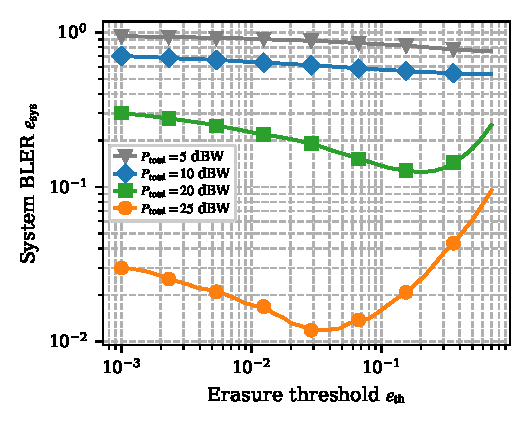
\includegraphics[width=0.7\columnwidth]{bler_vs_threshold.eps}\\
{\small \textbf{Fig.~\ref{fig:bler_vs_threshold}:} {\color{blue}System BLER versus erasure threshold
$\epsilon_{\mathrm{th}}$ at different transmit power levels.}}
\end{center}

In summary, the simulation results show that $\ldots$''
\end{quote}

We hope that the new threshold sensitivity figure clarifies the role of this parameter.

\vskip 0.2in
We greatly appreciate your valuable feedback and the time you have invested in evaluating our work. We are confident that the revisions effectively address all the concerns raised and enhance the overall quality of the manuscript.
%%%%%%%%%%%%%%%%%%%%%%%%%%%%%%%%%%%%%%%%%%%%%%%%%%%%%%%%%%%%%%%%%%%%%%